\newcommand{\bits}{\{0,1\}}
\newcommand{\bfu}{\mathbf{u}}
\newcommand{\bfv}{\mathbf{v}}
\newcommand{\bfp}{\mathbf{p}}
\newcommand{\bfz}{\mathbf{z}}
\newcommand{\bfx}{\mathbf{x}}
\newcommand{\bfy}{\mathbf{y}}

\newcommand{\bbZ}{\mathbb{Z}}
\newcommand{\calR}{\mathcal{R}}
\newcommand{\msf}{\mathsf}
\newcommand{\garble}[1]{\{\{ #1\}\}}

Today, we discuss garbled RAM, a paradigm for random access memory (RAM) secure multiparty computation (MPC). In particular, we initially look at garbled circuits implemented by Andrew Yao\cite{yao}, and then we discuss its extension into the garbling of RAM programs using ideas from recent sublinear computation construction \cite{epigram}\cite{nanogram} without increasing round complexity. 
\section{Secure Multiparty Computation}
While classical cryptography (encryption, authentication, etc.) is about securing communication, modern cryptography (ZKP, MPC, etc.) is about securing computation. 
Informally, the premise for MPC is a group of mutually distrusting parties, each with a private input. Their objective is to learn the result of an agreed-upon computation, such as an election, auction, etc. with the security guarantees being privacy (everyone only learns the output), input independence, and output consistency. MPC can be more formally defined using a simulator and corrupted parties. For a reference, see $\cite{Goyal}.$
\section{Yao's Garbled Circuits}
Yao's garbled circuits allow for circuit-based multi-party computation. 
For simplicity, we describe a two-party secure computation between Alice and Bob, who compute the result of a function $f(x,y)$ representable by a single gate taking in an input bit $x$ from Alice and an input bit $y$ from Bob. 
The truth table of this function is
\begin{center}
    \begin{tabular}{c|c|c}
         Alice's Input $x$ & Bob's Input $y$ & $f(x,y)$\\
         \hline
         0& 0 & $f(0,0)$ \\ 
         0& 1 & $f(0,1)$ \\ 
         1& 0 & $f(1,0)$ \\
         1& 1 & $f(1,1)$
    \end{tabular}
\end{center}.
In Yao's protocol, Alice acts as the "garbler," and Bob acts as the "evaluator."
Suppose that they agree on some encryption scheme $(G,E,D)$.
Alice writes out a garbled, encrypted truth table for Bob as follows:
\begin{mdframed}[innertopmargin=5pt, skipabove=\topskip, skipbelow=\topskip,align=left,nobreak=true]
\begin{enumerate}
    \item For input $x$, choose random crypto keys $A_0,A_1$. Symmetrically, for input $y,$ choose random crypto keys $B_0,B_1.$
    \item Encrypt each output with the corresponding keys. That is, for input $(x,y)$, Allice encrypts $E_{A_x}(E_{B_y}(f(x,y))).$
    \item Randomly permute the outputs and send to Bob.  
\end{enumerate}
\end{mdframed}
\newpage
Intuitively, if Bob can learn the correct keys $A_x,B_y$ without learning their shared input $(x,y),$ then Bob can only correctly decrypt the desired function output.
To do exactly this, we use an \textbf{oblivious transfer} (OT) protocol. 

In a 1-out-of-2-OT, Alice has two items $a_0, a_1$, where Bob wants to learn $a_b, b \in \{0,1\}.$

\begin{figure}
    \centering
    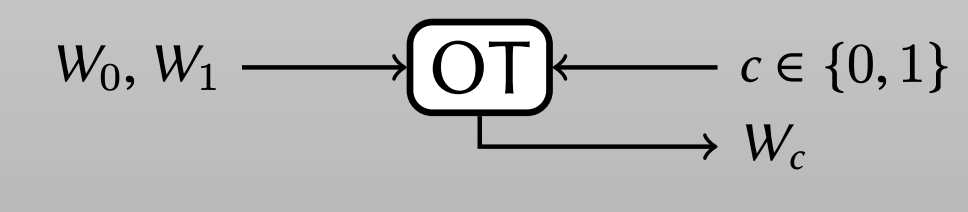
\includegraphics[scale=0.5]{OT.png}
    \caption{1-out-of-2-OT \cite{Rosulek_2018}}
    \label{fig:ot}
\end{figure}
In the protocol, Alice inputs $\beta_0, \beta_1$ and Bob inputs $\gamma$. At the end of the protocol, Alice learns nothing of Bob's bit $\gamma,$ and Bob learns $\beta_\gamma$ and nothing else.
For a detailed specification of OT protocols, see \cite{Goyal}.

One last technicality in this garbled circuit protocol is how will Bob know when he has decrypted the correct cipher? 
An easy solution to this is simply to prepend or append a string of 0s and have Bob check this. If we assume that we are using a secure encryption, then we have false positives with a negligible probability. Formally,
\begin{mdframed}[innertopmargin=5pt, skipabove=\topskip, skipbelow=\topskip,align=left,nobreak=true]
Modified Encryption
\begin{itemize}
    \item $\msf{Gen}(1^\lambda): k \leftarrow \{0,1\}^n$
    \item $\msf{Enc_k}(m): r \leftarrow \{0,1\}^n.$ Output $(r,(0^n || m) \oplus \msf{PRK_k}(r)$
    \item $\msf{Dec_k}(c_1,c_2):$ Compute $m_0||m_1 \leftarrow c_2 \oplus \msf{PRF}_k(c_1)$. If $m_0 = 0^n$, output $m_1.$ Else output $\perp.$
\end{itemize}
\end{mdframed}

Thus, the protocol is complete, where Alice will send a garbled truth table, Bob will request the correct keys via a 1-out-of-two OT, and Bob will successfully decode the correct output except with negligible probability.
\subsection{Extending to Many Gate Circuits}
The extension of this single gate protocol to a multi-gate protocol uses the same idea to propagate gate keys. 
Instead of simply returning the function output plaintext, every wire has two corresponding keys, where the communicated result from a gate is the next wire key.

For instance consider the 2-fan-in AND gate with input wire keys $A_0,A_1$ and $B_0,B_1$ and output wire keys $C_0,C_1.$ Then Alice's communicated table (before permuting) is illustrated by figure \ref{fig:garbAnd}.


\begin{figure}[!ht]
\centering
\resizebox{1\textwidth}{!}{%
\begin{circuitikz}
\tikzstyle{every node}=[font=\small]
\draw (2.25,10.75) to[short] (4,10.75);
\draw (2.25,10.25) to[short] (4,10.25);
\draw (4,10.75) node[ieeestd and port, anchor=in 1, scale=0.89](port){} (port.out) to[short] (7.25,10.5);
\node [font=\small] at (2.5,11.25) {$A_0,A_1$};
\node [font=\small] at (2.5,9.75) {$B_0,B_1$};
\node [font=\small] at (8.25,11.5) {$\substack{E_{A_0}\left(E_{B_0}\left(C_0\right)\right)\\E_{A_0}\left(E_{B_1}\left(C_0\right)\right)\\E_{A_1}\left(E_{B_0}\left(C_0\right)\right)\\E_{A_1}\left(E_{B_1}\left(C_1\right)\right)}$};
\end{circuitikz}
}
\caption{Key Propagation in a garbled AND Gate}

\label{fig:garbAnd}
\end{figure}


Thus, for arbitrary circuits, Bob will incrementally learn the wire keys corresponding only to the circuit computation on their input, until he learns the final function output.

In conclusion, 2PC can be performed using Yao's garbled circuit, which can be done in 2 rounds by having Alice send all the truth tables at once. 
\begin{figure}
    \centering
    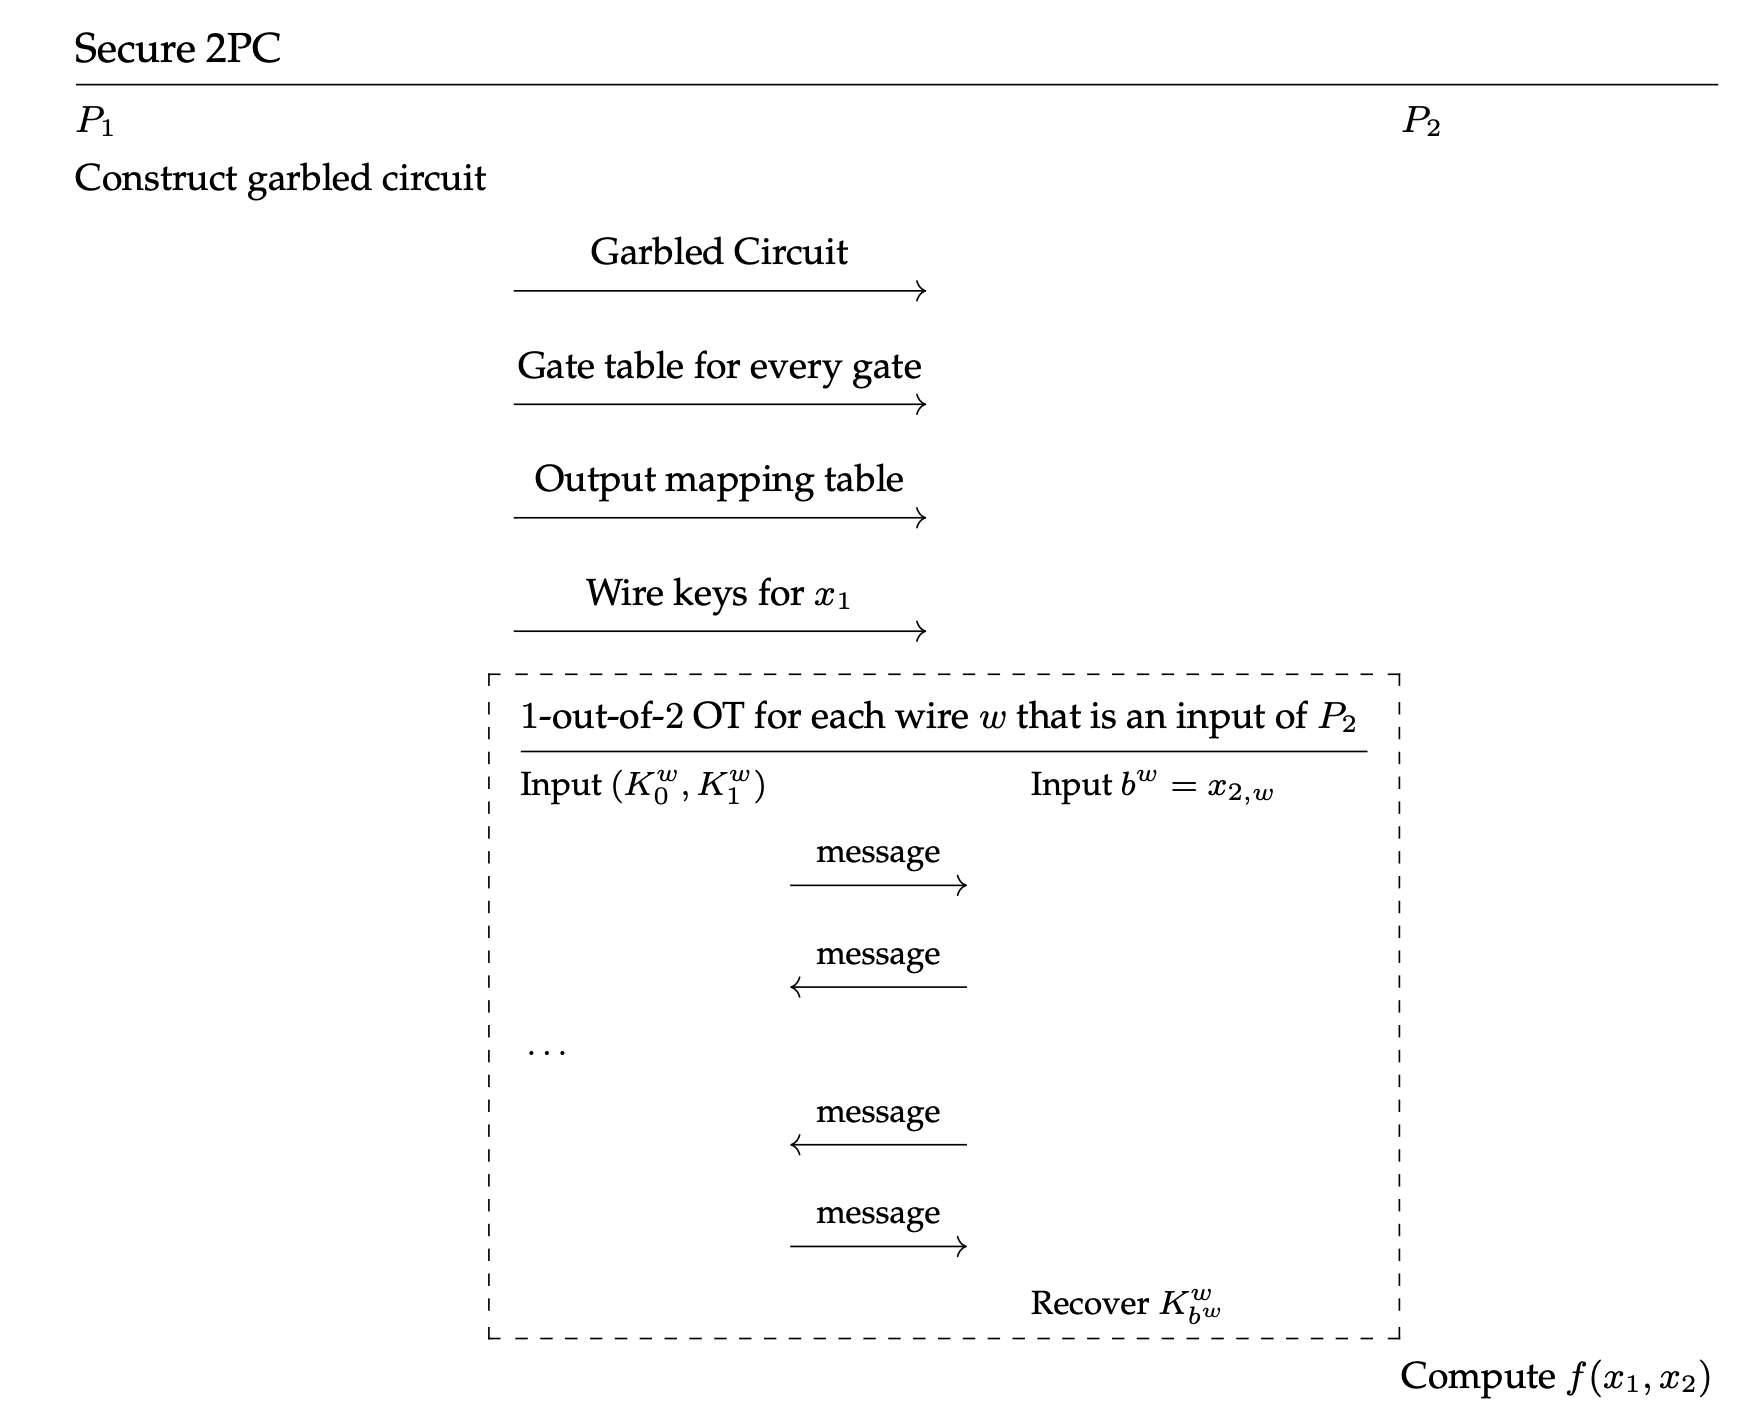
\includegraphics[scale=0.45]{2pc.png}
    \caption{2PC Protocol with Yao's Circuits}
    \label{fig:yao}
\end{figure}
\section{Garbled RAM}
Next, we discuss the problem of garbling RAM programs.
Many of the practical programs and functions (eg graph traversal) we care about rely on RAM. Since the accesses and writes of these programs are often dynamical and unpredictable in nature, they are not naively transformable into circuits without a large overhead. A naive translation of memory accesses to circuits is to implement a \textit{linear array circuit}, which takes in an access index $i$ and the memory array $A$, and outputs $A[i]$ via a linear scan. 

Thus, generically, if $T$ is the RAM program's run time and $n$ is the size of the memory array, then naive circuit transformation with linear access circuits gives us $O(Tn)$ run time. A main challenge of garbled RAM is doing better than linear blow-up by garbling these dynamical accesses with sublinear cost, while keeping the two-round complexity of the original garbled circuit. 

\subsection{RAM Model 2PC: ORAM + 2PC}
We start with a conceptually simpler protocol if we disregard the number of communication rounds.

Suppose that we have ORAM and 2PC protocols. Suppose that we have some non-oblivious RAM program between Alice and Bob. Then, we can apply an ORAM protocol to make it oblivious.

Now, by obliviousness, it is safe to reveal which memory addresses are accessed. We denote memory state of the program as $\msf{mem}$ with additive secret shares $\msf{st_0},st_1$ that Alice and Bob hold respectively.

Then Alice and Bob will emulate each step of the RAM program.
For every step of the program, the known read address is $\msf{addr}$. Alice reads $\msf{st_0}[\msf{addr}]$, and Bob reads $\msf{st_1}[\msf{addr}]$.

Then, they run a 2PC circuit protocol known as a \textit{next-step instruction circuit}, where Alice's input is $\msf{st_0}[\msf{addr}]$, and Bob's input is $\msf{st_1}[\msf{addr}]$. 
The output of this protocol is $\msf{wdata}_0, \msf{wdata}_1,\msf{waddr},\msf{raddr}$, where $\msf{wdata}_0, \msf{wdata}_1$ are secret shares of the write data for Alice and Bob, respectively, $\msf{waddr}$ is where the data is to be written, and $\msf{raddr}$ is the next read address.

Thus, this protocol will successfully implement garbled RAM, with the downside of increased round complexity. If the original program runs in time $T$, then using some practical ORAM, such as circuit ORAM, will have a $O(T\log^2 n)$ runtime.

% \subsubsection{Example: Database Querying}
% The memory state can be the database entries $\msf{DB}_0 \oplus \msf{DB}_1$ where Alice and Bob's inputs are secret shares of a query $q_0 \oplus q_1$. Then, they can compute querying function $f(q_0 \oplus q_1, \msf{DB}_0 \oplus \msf{DB}_1)$ using a 2PC protocol.

\subsection{Garbled RAM in Two Rounds}
The main challenge of garbled RAM is that the garbler cannot predict which memory locations are accessed at each time step.
To construct a garbled RAM protocol preserving Yao's round complexity, we will build tools to help us.
\subsubsection{Garbled Memory}
To work toward garbled RAM, we define an abstraction called \textit{ garbled memory}.
Suppose that we want to support $\msf{read(addr),write(addr,data)}$ and we allow ourselves to do this naively. That is, we are allowed to linear scan the memory to find and store the address to which we are reading/writing. 
In this case, the memory patterns are fixed since we just perform a linear scan every time. Also, this is easy to garble; say we have garbled memory under different labels $\msf{L}_{addr,t}$ in time step $t$ (in garbled circuits, labels are the wire keys, but this language reframes the problem of propogating keys as a conceptually simpler "label translation").
The garbler can just generate all the labels and then the evaluator will know which label to use to read the garbled data.
Although this incurs a linear cost to scan the garbled memory, this provides good intuition for the sublinear garbled RAM protocol.
\subsubsection{Garbled Stack}
Now, we work towards a more clever solution. Suppose that we want to garble a stack supporting two operations: $\msf{init(D)}$ and $\msf{pop(b)}$, where, 
\begin{mdframed}[innertopmargin=5pt, skipabove=\topskip, skipbelow=\topskip,align=left,nobreak=true]
Stack Interface
\begin{itemize}
    \item $\msf{init(D)}$: Initializes the stack with data $D$.
    \item $\msf{pop(b)}$: If $b = 0$, perform a fake pop (no state change) and output a dummy value. Otherwise, if $b = 1$, perform a real pop and return the top of the stack.
\end{itemize}
\end{mdframed}
If the garbler knows ahead of time which pops are real, then garbling this stack is again easy and predictable. Unfortunately, this will not be the case in our use of the garbled stack.

To garble a stack when we cannot predict the pop patterns, we observe that our stack is just a special case of a turing machine, where the head of the stack simply moves down or stays put! 
Thus, we can use an oblivious turing machine (OTM) protocol as discussed in previous lectures, which transforms the TM into a circuit with only $\log n$ factor overhead. That is, if our TM runs in time $T$ with memory array size $n,$ the circuit runs in time $O(T\log n)$.
\begin{figure}
    \centering
    \[\underbrace{\text{Stack}}_{T \text{ time}} \, \substack{\Longrightarrow\\ \text{ OTM }} \, \underbrace{\substack{\text{Oblivious Stack}\\ \text{(Circuit)}}}_{O(T\log n) \text{ time}}  \, \substack{\Longrightarrow\\\text{Yao}} \, \underbrace{\text{Garbled Stack}}_{O(T\log n) \text{ time}}\]
    \caption{Two-Round Stack to Garbled Stack, with labeled run times}
    \label{fig:transform}
\end{figure}
\subsection{Garbled Switch}
The last gadget we will construct is the \textit{garbled switch}. 
Our objective will be to garble a tree-based ORAM, like path-ORAM.
However, we run into the issue that the access paths are unpredictable, similar to our previous garbling problems. 
The garbled switch will provide us with the mechanism of making the tree-based ORAM garbled by providing the label switching functionality.


Let $\garble{x}_p$ denote x under a garbling with label $p$.
The gadget will consist of a parent node and two child nodes.


\begin{figure}
    \centering
    \begin{tikzpicture}
      % Nodes
      \draw [->, >=Stealth] (0,1) -- (0,.5);
      \node at (1,1.5) {$\garble{\msf{dir_t^E},\msf{data_t}}_{P_t}$};
      \node[circle, draw] (parent) at (0,0) {P};
      % \draw  (-.5,3) rectangle (-2,.5);
      \node[draw,align=center] at (-1.25,1.75) {$P_1$ \\ $\vdots$ \\ $P_m$};
      \node[circle, draw] (leftchild) at (-2,-3) {L};
      % \draw  (-2,0) rectangle (-3.5,-2.5);
      \node[draw,align=center] at (-2.75,-1.25) {$L_1$ \\ $\vdots$ \\ $L_m$};
      \node[circle, draw] (rightchild) at (2,-3) {R};
      % \draw  (2,0) rectangle (3.5,-2.5);
      \node[draw,align=center] at (2.75,-1.25) {$R_1$ \\ $\vdots$ \\ $R_m$};

      
    
      % Edges
      \draw (parent) -- (leftchild);
      \draw (parent) -- (rightchild);
    \end{tikzpicture}
    \caption{A Garbled Switch: Parent $P$ receives $\garble{\msf{dir_t^E}_{p_t}, \msf{data_t}}$ to route. Parent $P$ has labels $P_1,\dots,P_m$, left child $L$ has labels $L_1,\dots,L_m$, and right child $R$ has labels $R_1,\dots,R_m$.}
    \label{fig:switch}
\end{figure}

At time step $t$, there is incoming data $\garble{\msf{dir_t^E}, \msf{data_t}}_{p_t}$ where $\msf{dir_t^E} \in \{0,1\}$ is the direction of routing ($0$ for left child, $1$ for right child), $\msf{data_t}$ is the data to route. 
Here, we also use the $(.)^E$ superscript notation to denote that the variable does not need to be private. In the ORAM-tree, recall that it is ok for the direction to be known (and is necessary for efficiency). 

The parent will hold labels $P_1,\dots,P_m$, the left child will hold labels $L_1,\dots,L_m$, and the right child will hold labels $R_1,\dots,R_m$, where $m$ is the maximum number of times the parent is invoked. 
The idea is that during the first time data is routed to the left node, it should be encoded under label $L_1$ ie $\garble{\msf{data_t}}_{L_1}$, during the second time $L_2$ ie $\garble{\msf{data_t}}_{L_2}$, and so on$\dots$.
Thus, each node will keep track of a local time corresponding to each time it has been invoked so that we can apply a label that both parent and child agree with.
Then, the child will be able to understand the garbled data and will be able to do its garbled computation on it.

We can construct a garbled switch protocol for the evaluator using two garbled stack to store corresponding labels,
\begin{mdframed}[innertopmargin=5pt, skipabove=\topskip, skipbelow=\topskip,align=left,nobreak=true]
Garbled Switch Protocol. 

Suppose Evaluator has labels $L_1,\dots,L_m,R_1,\dots,R_m$ and garbling encoding function $\msf{garbenc}$:
\begin{enumerate}
    \item Evaluator initializes two stacks:
    \begin{align*}
        \msf{stackL} &\leftarrow \msf{GStack.init}(L_1,\dots,L_m),\\
        \msf{stackR} &\leftarrow \msf{GStack.init}(R_1,\dots,R_m)
    \end{align*}
    \item In parent time step $t,$ suppose the data is to be routed to the left child, whose local time is $v.$ 
    Evaluator runs:
    \begin{align*}
    \garble{\Bar{L}}_{P_t} &\leftarrow \msf{StackL.pop}(\garble{1 - dir^E_t}_{P_t}) \\
    \garble{\Bar{R}} &\leftarrow \msf{StackR.pop}(\garble{dir^E_t}_{P_t}),\\
    \garble{data_t}_{L_v} &\leftarrow \msf{garbenc}(\garble{data_t}_{P_t},\garble{\Bar{L}}_{P_t})
    \end{align*}    
    Note that $\garble{\Bar{R}}$ is garbled under some garbage label.
    \end{enumerate}
\end{mdframed}
The protocol uses a garbling encoding function $\msf{garbenc}$, which can be represented by an efficient garbled circuit, since its input and output are predictable (labels are only dependent on time). 
Likewise, the stacks are also predicatable, so there are no problems garbling.

\subsubsection{Garbled Switches $\rightarrow$ ORAM Tree}
With the garbled switch, we can combine many of them to make arbitrary trees. 
Our last step in garbling ORAM is to provide a procedure for reading and writing in this tree.

Suppose we have a path-ORAM tree, where every node implements a garbled switch and a constant-sized garbled bucket implemented with garbled memory (constant-size make linear scans cheap).

\subsubsection{Garbled Reads}
Recall in a nongarbled path-ORAM, if we already know the path denoted by $\msf{leaf},$ along with read labels $\msf{RdL_0},\dots,\msf{RdL_D}$, where $D$ is the depth, and the read address $\msf{addr}$, we will search for $\msf{addr}$ along the path.
If the element resides in the root bucket, then it will return the element garbled under $\msf{RdL_0}$. If the element is in the second node in the path, then it will return the element garbled under $\msf{RdL_1}$, and so on$\dots$.
However, the next-instruction circuit will be garbled under the global time label (the root local time), so in order for the output to work with the next-instruction circuit, we also need to pass the read labels down the path, so every node will know what the output label should be.
\begin{mdframed}[innertopmargin=5pt, skipabove=\topskip, skipbelow=\topskip,align=left,nobreak=true]
Garbled path-ORAM Read Summary:
\begin{enumerate}
    \item Garble the entire state of the read labels, path, and address along the path, so every node along the path can read the garbled data under the language it understands.
    \item At each node along the path,  check the bucket for the address and output either the answer or garbage under the correct output label.
    \item Once the next-instruction circuit receives the $O(\log n)$ garbled results under the output label, it can decipher the real result and proceed to the next instruction.
    \end{enumerate}
\end{mdframed}

\subsubsection{Garbled Writes}
To implement writing, we need to implement path-ORAM eviction.
Recall that eviction takes place only along a path.
We think of eviction in a different but equivalent way: suppose that every node along the path outputs some $\msf{metadata}$. 
Then, for an eviction protocol, we have some circuit $f$ taking in the metadata and outputting an eviction plan.
For every node in the path, we use some circuit $g$ that takes its bucket, eviction plan, and the data it has received and outputs its new bucket, eviction plan, and the data to pass on.

With this view, we can implement garbled eviction in the same way as garbled reads. We will pass down data along the path, every node will output some metadata garbled under some desired label (like the read labels), and the garbled metadata will be passed to a next-instruction circuit in a label it understands.

\begin{mdframed}[innertopmargin=5pt, skipabove=\topskip, skipbelow=\topskip,align=left,nobreak=true]
Garbled path-ORAM Write(Eviction) Summary:

Think of path-ORAM eviction as follows,
\begin{enumerate}
    \item Suppose that every node along the path stores $\msf{metadata}$, and that we have circuit $f$ such that:
    \[f(\msf{metadata}) \rightarrow \msf{eviction plan}\]
    \item At each node along the path, we have circuit $g$ outputting:
    \[\substack{\msf{bucket'}\\\msf{eviction plan}\\ \text{data to pass on}} \leftarrow g(\msf{bucket}, \msf{eviction plan}, \text{data recieved})\]
    \item The next-instruction circuit takes the data and outputs the next instruction.  
    \end{enumerate}
    Then, the garbling is the same as reading.
\end{mdframed}
